In this chapter we present the different tests that were performed to compare the capabilities of the old and new methods. For each test, the results of both methods of discretization are compared.

In total, four kinds of tests were conducted:
\begin{itemize}
	\item Invariance
	\item Image reconstruction
	\item Image recognition
	\item Template matching
\end{itemize}

\section{Test images}\label{sec:test_images}
The images for testing were acquired from multiple online image libraries. The Lenna and Pepper images~\cite{usc_sipi} (shown on Figure~\ref{fig:lena_pepper_original}) were used to test image reconstruction as well as to demonstrate the different points systems.

\begin{figure}[tbp]
    \begin{subfigure}{0.49\textwidth}
        \centering
    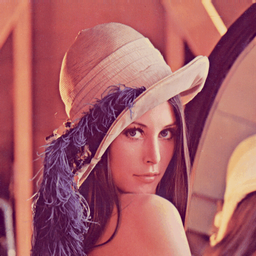
\includegraphics[width=128pt]{figures/lenna_color_256.png}
    \caption{}
	\end{subfigure}
	\begin{subfigure}{0.49\textwidth}
        \centering
    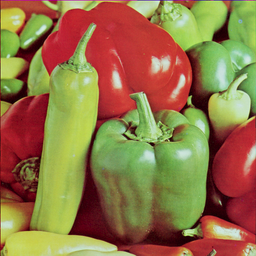
\includegraphics[width=128pt]{figures/pepper_color_256.png}
    \caption{}
	\end{subfigure}
	\caption{The Lenna and Pepper images}
	\label{fig:lena_pepper_original}
\end{figure}

For the image recognition tests, two sets of images were used. The first set consists of 14 images chosen from the Columbia Object Image Library (COIL-100)~\cite{coil}, shown on Figure~\ref{fig:coil_original}. These images are originally $128 \times 128$ pixels, but they were placed on a $204 \times 204$ black background so that the rotated, scaled and translated versions of the images remain completely within these dimensions. 

A set of 1008 rotated images was created by rotating each of the 14 images by a degree $\alpha\in\{0,5,10,\ldots,350,355\}$. Some examples of the extended and rotated images are shown on Figure~\ref{fig:coil_rot}.

Another set of 1176 rotated, scaled and translated images was created by translating each image by -11 pixels in the $x$ direction and 9 pixels in the $y$ direction. Then the translated images were rotated by $\alpha \in \{0,30,60,\ldots,300,330\}$. Finally, each rotated and translated image was scaled by $\lambda \in \{0.5, 0.75, \ldots, 1.75, 2\}$. When either scaling or rotation required, bilinear interpolation was used.
Some examples of the RST transformed images are shown on Figure~\ref{fig:coil_rst}.

\begin{figure}[tbp]
    \begin{subfigure}{80pt}
        \centering
    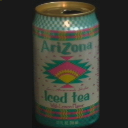
\includegraphics[width=\textwidth]{figures/coil_original/7.png}
    \caption{}
	\end{subfigure}
	\begin{subfigure}{80pt}
        \centering
    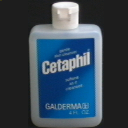
\includegraphics[width=\textwidth]{figures/coil_original/13.png}
    \caption{}
	\end{subfigure}
	\begin{subfigure}{80pt}
        \centering
    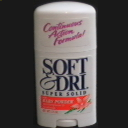
\includegraphics[width=\textwidth]{figures/coil_original/22.png}
    \caption{}
	\end{subfigure}
	\begin{subfigure}{80pt}
        \centering
    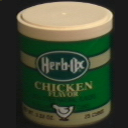
\includegraphics[width=\textwidth]{figures/coil_original/26.png}
    \caption{}
	\end{subfigure}
	\begin{subfigure}{80pt}
        \centering
    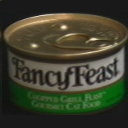
\includegraphics[width=\textwidth]{figures/coil_original/29.png}
    \caption{}
	\end{subfigure}
	\begin{subfigure}{80pt}
        \centering
    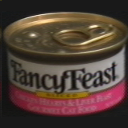
\includegraphics[width=\textwidth]{figures/coil_original/32.png}
    \caption{}
	\end{subfigure}
	\begin{subfigure}{80pt}
        \centering
    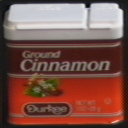
\includegraphics[width=\textwidth]{figures/coil_original/39.png}
    \caption{}
	\end{subfigure}
	\begin{subfigure}{80pt}
        \centering
    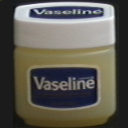
\includegraphics[width=\textwidth]{figures/coil_original/55.png}
    \caption{}
	\end{subfigure}
	\begin{subfigure}{80pt}
        \centering
    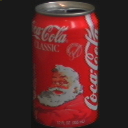
\includegraphics[width=\textwidth]{figures/coil_original/62.png}
    \caption{}
	\end{subfigure}
	\begin{subfigure}{80pt}
        \centering
    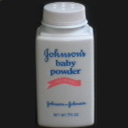
\includegraphics[width=\textwidth]{figures/coil_original/64.png}
    \caption{}
	\end{subfigure}
	\begin{subfigure}{80pt}
        \centering
    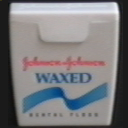
\includegraphics[width=\textwidth]{figures/coil_original/65.png}
    \caption{}
	\end{subfigure}
	\begin{subfigure}{80pt}
        \centering
    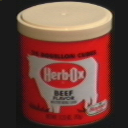
\includegraphics[width=\textwidth]{figures/coil_original/71.png}
    \caption{}
	\end{subfigure}
	\begin{subfigure}{80pt}
        \centering
    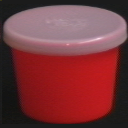
\includegraphics[width=\textwidth]{figures/coil_original/95.png}
    \caption{}
	\end{subfigure}
	\begin{subfigure}{80pt}
        \centering
    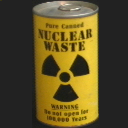
\includegraphics[width=\textwidth]{figures/coil_original/99.png}
    \caption{}
    \end{subfigure}
	\caption{The 14 selected images from the Columbia Object Image Library (COIL-100)}
	\label{fig:coil_original}
\end{figure}

\begin{figure}[tbp]
	\begin{subfigure}{0.30\textwidth}
        \centering
    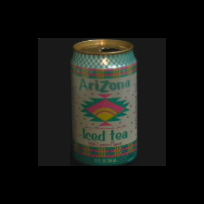
\includegraphics[width=102pt]{figures/coil_rot/7r0.png}
    \caption{$\alpha=0^{\circ}$}
	\end{subfigure}
	\begin{subfigure}{0.30\textwidth}
        \centering
    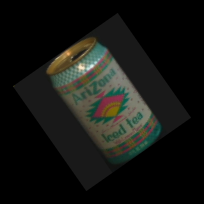
\includegraphics[width=102pt]{figures/coil_rot/7r35.png}
    \caption{$\alpha=35^{\circ}$}
	\end{subfigure}
	\begin{subfigure}{0.30\textwidth}
        \centering
    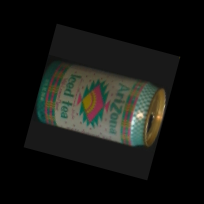
\includegraphics[width=102pt]{figures/coil_rot/7r255.png}
    \caption{$\alpha=255^{\circ}$}
	\end{subfigure}
	\caption{Some extended and rotated images from COIL}
	\label{fig:coil_rot}
\end{figure}

\begin{figure}[tbp]
	\begin{subfigure}{0.29\textwidth}
        \centering
    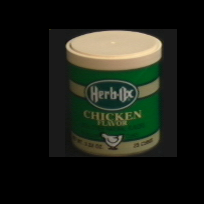
\includegraphics[width=102pt]{figures/coil_rst/26x-11y9r0s1_0.png}
    \caption{$\alpha=0^{\circ}$, $\lambda=1$}
	\end{subfigure}
	\begin{subfigure}{0.28\textwidth}
        \centering
    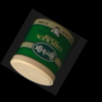
\includegraphics[width=51pt]{figures/coil_rst/26x-11y9r150s0_5.png}
    \caption{$\alpha=150^{\circ}$, $\lambda=0.5$}
	\end{subfigure}
	\begin{subfigure}{0.40\textwidth}
        \centering
    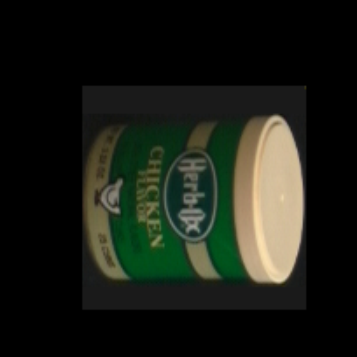
\includegraphics[width=153pt]{figures/coil_rst/26x-11y9r270s1_75.png}
    \caption{$\alpha=270^{\circ}$, $\lambda=1.5$}
	\end{subfigure}
	\caption{Some RST transformed images from COIL. All images are translated by $\Delta x = -11$, $\Delta y = 9$}
	\label{fig:coil_rst}
\end{figure}

Another set of 13 images was acquired from the Amsterdam Library of Object Images (ALOI)~\cite{aloi}. These are shown on Figure~\ref{fig:aloi_original}. Originally, these size of these images was $768 \times 576$ pixels, but the were downscaled to $96 \times 72$ and subsequently extended to $152 \times 128$ by placing the images on a black background. Similarly to the test sets created using the COIL-100 images, the ALOI images were also translated, rotated and scaled, yielding a set of 1092 RST transformed images. The parameters of the transformation were the same as for the COIL-100 images, except for the translation, where $\Delta x = 8$ and $\Delta y = 5$ was used.

\begin{figure}[tbp]
    \begin{subfigure}{80pt}
        \centering
    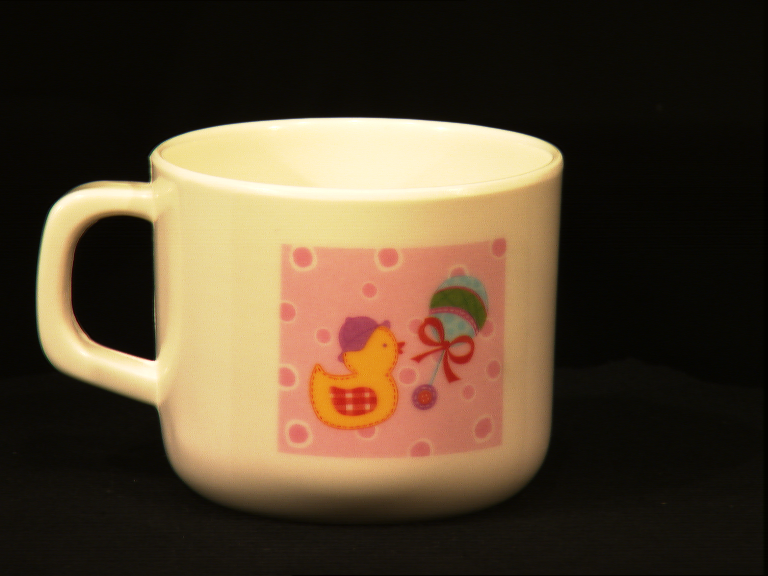
\includegraphics[width=\textwidth]{figures/aloi_original/36.png}
    \caption{}
	\end{subfigure}
	\begin{subfigure}{80pt}
        \centering
    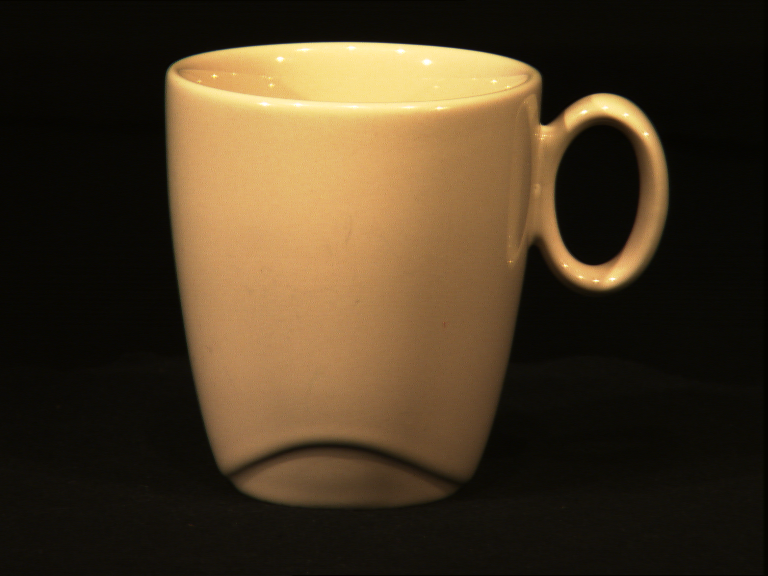
\includegraphics[width=\textwidth]{figures/aloi_original/125.png}
    \caption{}
	\end{subfigure}
	\begin{subfigure}{80pt}
        \centering
    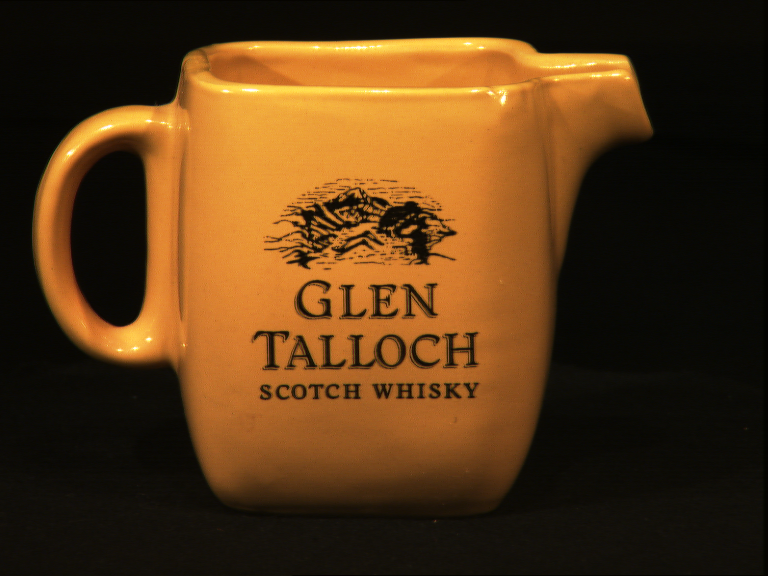
\includegraphics[width=\textwidth]{figures/aloi_original/127.png}
    \caption{}
	\end{subfigure}
	\begin{subfigure}{80pt}
        \centering
    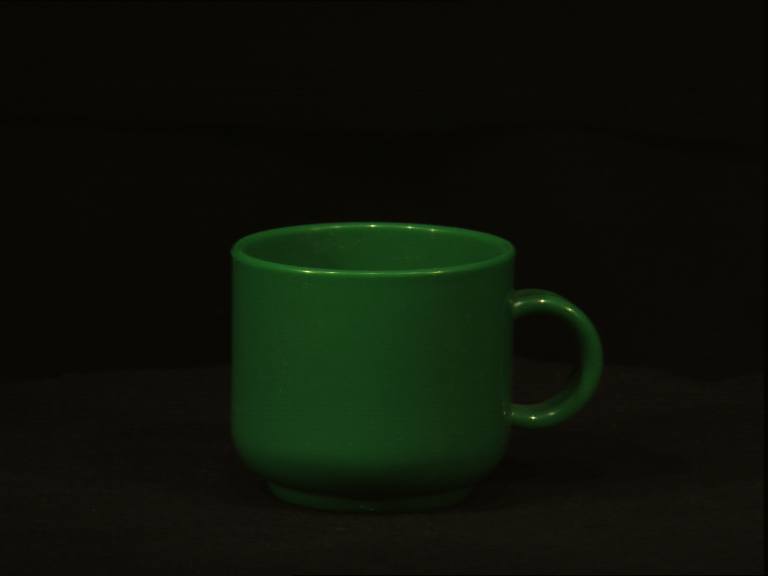
\includegraphics[width=\textwidth]{figures/aloi_original/153.png}
    \caption{}
	\end{subfigure}
	\begin{subfigure}{80pt}
        \centering
    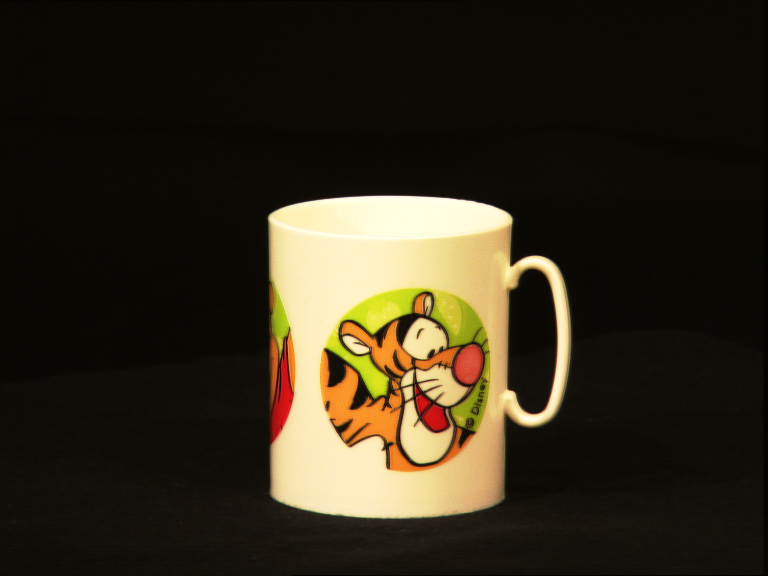
\includegraphics[width=\textwidth]{figures/aloi_original/157.png}
    \caption{}
	\end{subfigure}
	\begin{subfigure}{80pt}
        \centering
    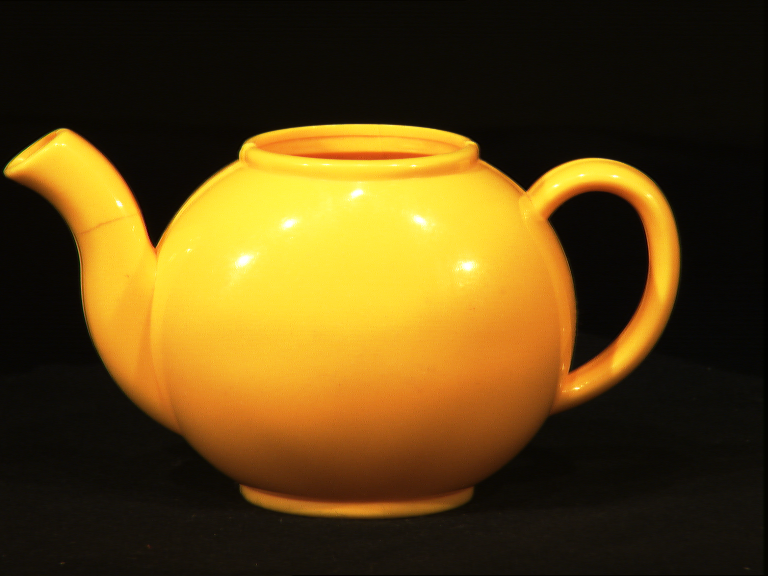
\includegraphics[width=\textwidth]{figures/aloi_original/161.png}
    \caption{}
	\end{subfigure}
	\begin{subfigure}{80pt}
        \centering
    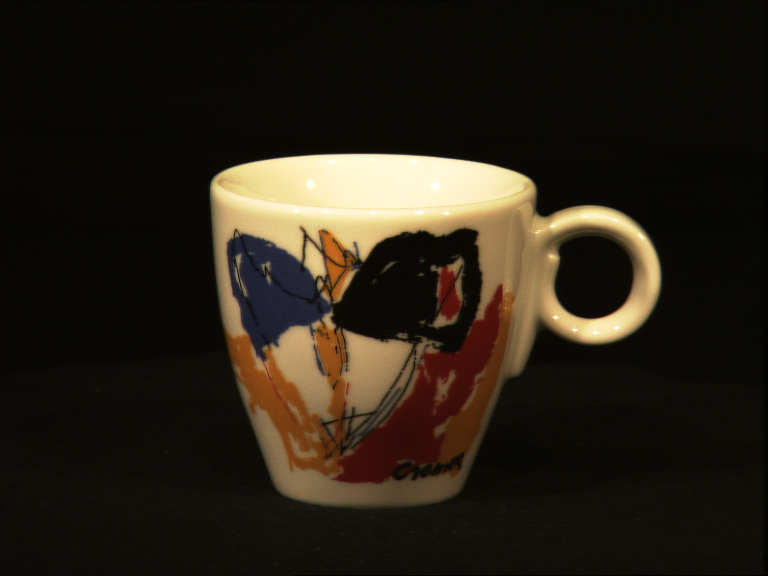
\includegraphics[width=\textwidth]{figures/aloi_original/259.png}
    \caption{}
	\end{subfigure}
	\begin{subfigure}{80pt}
        \centering
    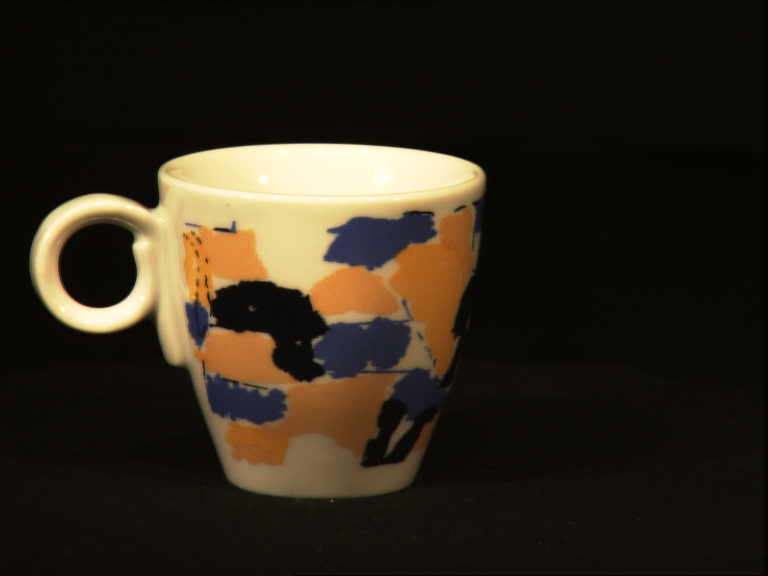
\includegraphics[width=\textwidth]{figures/aloi_original/262.png}
    \caption{}
	\end{subfigure}
	\begin{subfigure}{80pt}
        \centering
    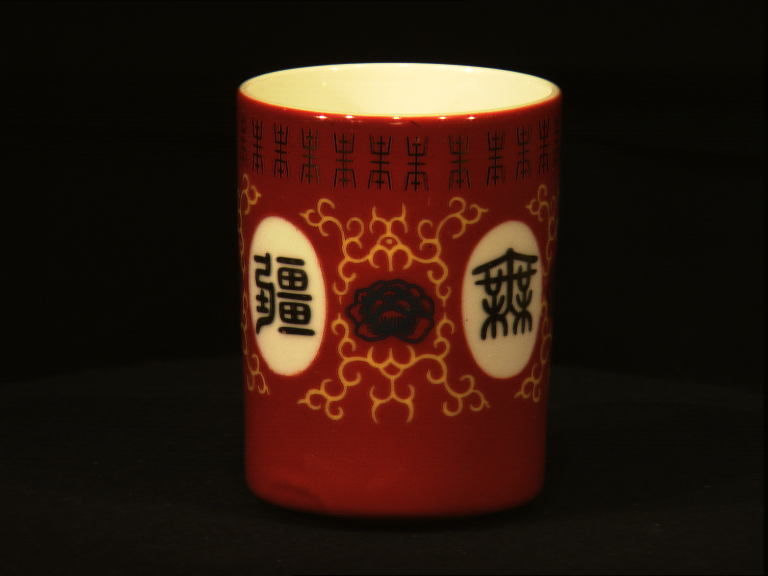
\includegraphics[width=\textwidth]{figures/aloi_original/308.png}
    \caption{}
	\end{subfigure}
	\begin{subfigure}{80pt}
        \centering
    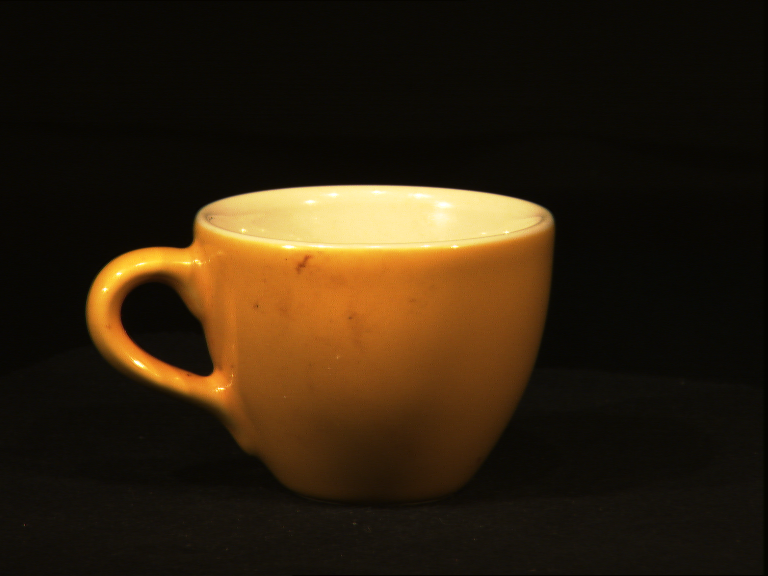
\includegraphics[width=\textwidth]{figures/aloi_original/507.png}
    \caption{}
	\end{subfigure}
	\begin{subfigure}{80pt}
        \centering
    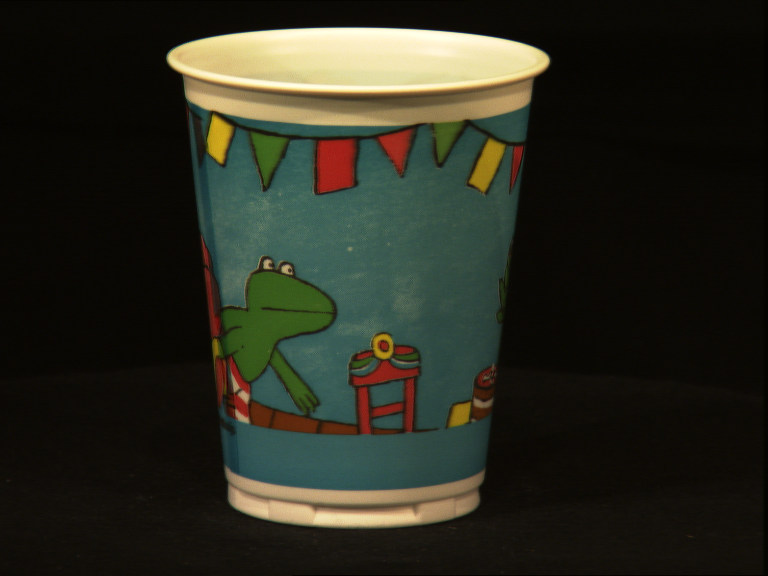
\includegraphics[width=\textwidth]{figures/aloi_original/514.png}
    \caption{}
	\end{subfigure}
	\begin{subfigure}{80pt}
        \centering
    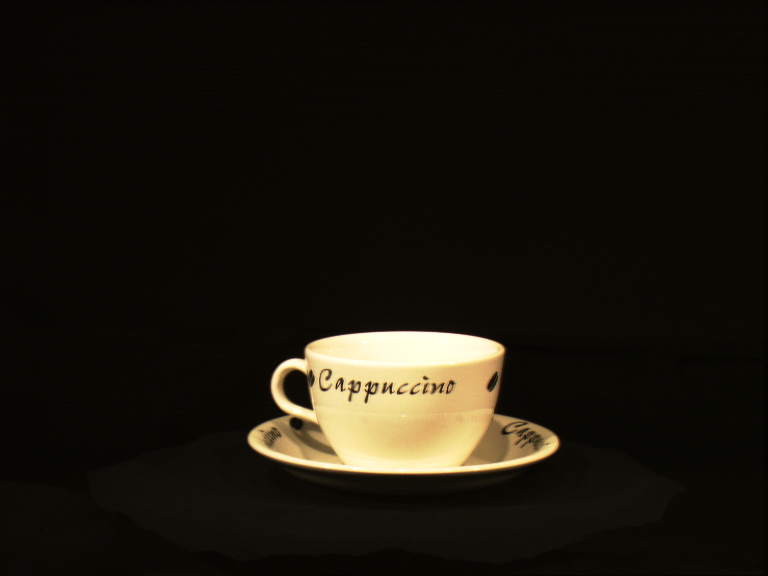
\includegraphics[width=\textwidth]{figures/aloi_original/774.png}
    \caption{}
	\end{subfigure}
	\begin{subfigure}{80pt}
        \centering
    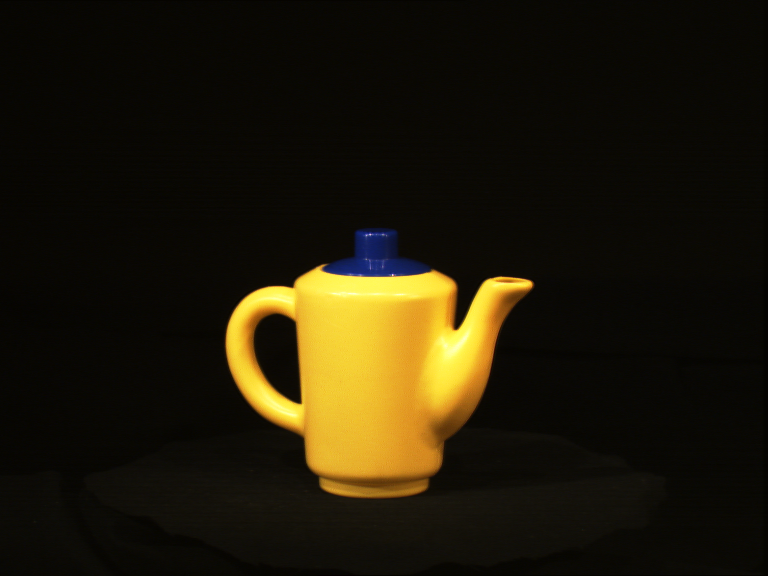
\includegraphics[width=\textwidth]{figures/aloi_original/875.png}
    \caption{}
	\end{subfigure}
	\caption{The 13 selected images from the Amsterdam Library of Object Images (ALOI)}
	\label{fig:aloi_original}

\end{figure}

\section{Invariance test}
In order to test the invariance of the quaternion Zernike moment invariants with respect to rotation, scaling and translation, the QZMIs of order 1 to 4 were calculated for a given image and all of its RST transformations. Then, the modulus of these QZMIs was calculated, as well as the mean ($\mu$), standard deviation ($\sigma$) and $\frac{\sigma}{\mu}$ for the same moment of all transformed images.

\begin{figure}[tbp]
	\begin{subfigure}{0.4\textwidth}
        \centering
    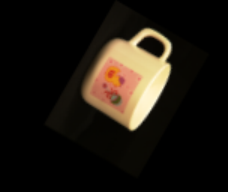
\includegraphics[width=150pt]{figures/inv_img/36x8y5r240s1_5.png}
	\caption{}\label{fig:inv_img1}
	\end{subfigure}
	\begin{subfigure}{0.29\textwidth}
        \centering
    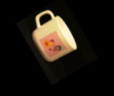
\includegraphics[width=75pt]{figures/inv_img/36x8y5r300s0_75.png}
    \caption{}\label{fig:inv_img2}
	\end{subfigure}
	\begin{subfigure}{0.29\textwidth}
        \centering
    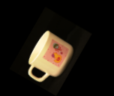
\includegraphics[width=75pt]{figures/inv_img/36x8y5r60s0_75.png}
    \caption{}\label{fig:inv_img3}
	\end{subfigure}
	\begin{subfigure}{0.3\textwidth}
        \centering
    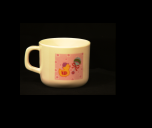
\includegraphics[width=100pt]{figures/inv_img/36x8y5r0s1_0.png}
    \caption{}\label{fig:inv_img4}
	\end{subfigure}
	\begin{subfigure}{0.3\textwidth}
        \centering
    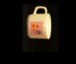
\includegraphics[width=50pt]{figures/inv_img/36x8y5r270s0_5.png}
    \caption{}\label{fig:inv_img5}
	\end{subfigure}
	\begin{subfigure}{0.3\textwidth}
        \centering
    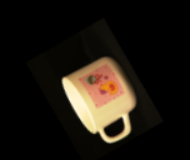
\includegraphics[width=125pt]{figures/inv_img/36x8y5r120s1_25.png}
    \caption{}\label{fig:inv_img6}
	\end{subfigure}
	\caption{The images with different rotation and scale, which are used to test the invariance of the methods.}
	\label{fig:inv_img}
\end{figure}

\subsection{Results}
The modulus of the QZMIs for the transformed images shown on Figure~\ref{fig:inv_img} is shown in Table~\ref{tab:inv_old} for the old method of discretization and in Table~\ref{tab:inv_new} for the new, proposed method of discretization. The coefficient of variation ($\frac{\sigma}{\mu}$) shows that using both methods, the moments are invariant to RST transformation. The only rows where $\frac{\sigma}{\mu}$ is higher are the ones where the modulus of the moment is very close to zero, and thus small numerical errors impact this number significantly. Comparing the two methods, the proposed one yields slightly lower values for the coefficient of variation for all moments.

\begin{table}
	\centering
\begin{tabular}{| c || c | c | c | c | c | c || c | } \hline
& Fig.\ref{fig:inv_img1} & Fig.\ref{fig:inv_img2} & Fig.\ref{fig:inv_img3} & Fig.\ref{fig:inv_img4} & Fig.\ref{fig:inv_img5} & Fig.\ref{fig:inv_img6} & $\frac{\sigma}{\mu}$ \\ \hline\hline
$|\overline{\Psi}_{1,1}^1|$ & 1.50e-2 & 1.58e-2 & 1.54e-2 & 1.61e-2 & 1.58e-2 & 1.49e-2 & 3.73\% \\ \hline
$|\overline{\Psi}_{2,0}^0|$ & 2.965 & 2.964 & 2.964 & 2.963 & 2.964 & 2.965 & 0.028\% \\ \hline
$|\overline{\Psi}_{2,2}^0|$ & 8.793 & 8.785 & 8.789 & 8.783 & 8.786 & 8.794 & 0.057\% \\ \hline
$|\overline{\Psi}_{2,2}^2|$ & 1.50e-4 & 1.65e-4 & 1.57e-4 & 1.69e-4 & 1.65e-4 & 1.47e-4 & 6.87\% \\ \hline
$|\overline{\Psi}_{3,1}^1|$ & 5.91e-2 & 6.25e-2 & 6.09e-2 & 6.34e-2 & 6.22e-2 & 5.89e-2 & 3.71\%  \\ \hline
$|\overline{\Psi}_{3,3}^1|$ & 0.233 & 0.247 & 0.241 & 0.250 & 0.246 & 0.233 & 3.69\% \\ \hline
$|\overline{\Psi}_{3,3}^3|$ & 1.43e-6 & 1.61e-6 & 1.50e-6 & 1.67e-6 & 1.62e-6 & 1.38e-6 & 9.40\% \\ \hline
$|\overline{\Psi}_{4,0}^0|$ & 4.827 & 4.821 & 4.824 & 4.820 & 4.822 & 4.828 & 0.086\% \\ \hline
$|\overline{\Psi}_{4,2}^0|$ & 14.316 & 14.291 & 14.302 & 14.284 & 14.292 & 14.318 & 0.114\% \\ \hline
$|\overline{\Psi}_{4,2}^2|$ & 7.39e-4 & 8.13e-4 & 7.74e-4 & 8.35e-4 & 8.12e-4 & 7.26e-4 & 6.85\% \\ \hline
$|\overline{\Psi}_{4,4}^0|$ & 23.309 & 23.249 & 23.276 & 23.232 & 23.251 & 23.314 & 0.171\% \\ \hline
$|\overline{\Psi}_{4,4}^2|$ & 3.64e-3 & 4.00e-3 & 3.81e-3 & 4.11e-3 & 4.00e-3 & 3.58e-3 & 6.83\% \\ \hline
$|\overline{\Psi}_{4,4}^4|$ & 1.28e-8 & 1.52e-8 & 1.39e-8 & 1.59e-8 & 1.51e-8 & 1.25e-8 & 12.00\% \\ \hline
\end{tabular}
\caption{The modulus of QZMIs using the old method for discretization. Note that $\frac{\sigma}{\mu}$ was calculated using the QZMIs for all transformation of the image, not juts the values shown in the table.}
\label{tab:inv_old}
\end{table}

\begin{table}
	\centering
\begin{tabular}{| c || c | c | c | c | c | c || c | } \hline
& Fig.\ref{fig:inv_img1} & Fig.\ref{fig:inv_img2} & Fig.\ref{fig:inv_img3} & Fig.\ref{fig:inv_img4} & Fig.\ref{fig:inv_img5} & Fig.\ref{fig:inv_img6} & $\frac{\sigma}{\mu}$ \\ \hline\hline
$|\overline{\Psi}_{1,1}^1|$ & 1.49e-2 & 1.58e-2 & 1.54e-2 & 1.60e-2 & 1.57e-2 & 1.49e-2 & 3.72\% \\ \hline
$|\overline{\Psi}_{2,0}^0|$ & 2.965 & 2.964 & 2.964 & 2.963 & 2.964 & 2.965 & 0.028\%\\ \hline
$|\overline{\Psi}_{2,2}^0|$ & 8.793 & 8.785 & 8.789 & 8.783 & 8.786 & 8.793 & 0.056\%\\ \hline
$|\overline{\Psi}_{2,2}^2|$ & 1.49e-4 & 1.64e-4 & 1.55e-4 & 1.68e-4 & 1.63e-4 & 1.47e-4 & 6.82\%\\ \hline
$|\overline{\Psi}_{3,1}^1|$ & 5.90e-2 & 6.25e-2 & 6.08e-2 & 6.33e-2 & 6.21e-2 & 5.89e-2 & 3.70\%\\ \hline
$|\overline{\Psi}_{3,3}^1|$ & 0.233 & 0.247 & 0.240 & 0.250 & 0.245 & 0.233 & 3.68\%\\ \hline
$|\overline{\Psi}_{3,3}^3|$ & 1.41e-6 & 1.61e-6 & 1.48e-6 & 1.65e-6 & 1.60e-6 & 1.37e-6 & 9.32\%\\ \hline
$|\overline{\Psi}_{4,0}^0|$ & 4.828 & 4.821 & 4.824 & 4.820 & 4.822 & 4.828 & 0.085\%\\ \hline
$|\overline{\Psi}_{4,2}^0|$ & 14.317 & 14.291 & 14.304 & 14.286 & 14.293 & 14.318 & 0.113\%\\ \hline
$|\overline{\Psi}_{4,2}^2|$ & 7.35e-4 & 8.13e-4 & 7.68e-4 & 8.29e-4 & 8.07e-4 & 7.25e-4 & 6.80\%\\ \hline
$|\overline{\Psi}_{4,4}^0|$ & 23.312 & 23.249 & 23.279 & 23.236 & 23.254 & 23.314 & 0.170\%\\ \hline
$|\overline{\Psi}_{4,4}^2|$ & 3.62e-3 & 4.00e-3 & 3.79e-3 & 4.09e-3 & 3.98e-3 & 3.58e-3 & 6.78\%\\ \hline
$|\overline{\Psi}_{4,4}^4|$ & 1.28e-8 & 1.52e-8 & 1.37e-8 & 1.56e-8 & 1.50e-8 & 1.24e-8 & 11.94\%\\ \hline
\end{tabular}
\caption{The modulus of QZMIs using the new method for discretization. Note that $\frac{\sigma}{\mu}$ was calculated using the QZMIs for all transformation of the image, not juts the values shown in the table.}
\label{tab:inv_new}
\end{table}

\section{Image reconstruction}
As described in Section~\ref{sec:qzm}, the quaternion Zernike moments of an image can be used to approximately reconstruct the original image using the formulas in (\ref{eq:qzm_reconstruction}). This reconstruction requires QZMs of up to a finite degree $M$.

In order to calculate the reconstructed discrete image, the 
$$
f(r_{x,y},\theta_{x,y}) \approx \sum_{n=0}^{M}\sum_{m=-n}^{n}Z_{n,m}^R(f)R_{n,m}(r_{x,y})e^{\bm{\mu}m\theta_{x,y}}
$$
formula was used for each pixel with image coordinates $(x,y)$, where $(r_{x,y},\theta_{x,y})$ are the polar coordinates obtained by performing the linear transformation of the image onto the unit disk, using the transformation shown on Figure~\ref{fig:transform1} (\textit{tf\textsubscript{1}}) for the old method and the transformation shown on Figure~\ref{fig:transform2} (\textit{tf\textsubscript{2}}) for the new one. The reason for this difference in transformation is that for the proposed discrete orthogonal points system, the interpolated pixel values are calculated using \textit{tf\textsubscript{2}}, while conventionally for (quaternion) Zernike moments, \textit{tf\textsubscript{1}} is used~\cite{qzmi}.

To measure the error of the reconstruction the normalized mean squared error ($\varepsilon^2$) was used. If $f(x,y)$ is the original and $\widehat{f}(x,y)$ is the reconstructed image, both with size $N \times N$, then the normalized mean squared error is defined as:
\begin{gather*}
    \varepsilon^2 = \frac{\displaystyle \sum_{x=1}^N\sum_{y=1}^N \left|f(x,y) - \widehat{f}(x,y)\right|^2}{\displaystyle \sum_{x=1}^N\sum_{y=1}^N \left|f(x,y)\right|^2}
\end{gather*}

In the cases, where \textit{tf\textsubscript{2}} is used only the part of the image falling inside the unit circle is reconstructed and thus the mean squared error is calculated over only this part of the image.

For the new method of discretization the number of points on the unit disk was chosen to be approximately the same as the number of pixels falling inside the inscribed circle of the image. 

\subsection{Results}
Image reconstruction was performed for both the Lena and the Pepper images, using image sizes ranging from $64\times 64$ up to $256 \times 256$. Depending on the size of the image, QZMs of up to degree 350 were used reconstruct the image. However, in the case of smaller images, for example a $64\times 64$ image, only QZMs of up to 100 degree could be used, as using higher degrees would result in trying to extract more information from the original image than there is information contained in the pixel values, thus increasing the error of reconstruction. This phenomenon is visible, for example on Figure~\ref{fig:reconstruction_new} for the $64 \times 64$ Lenna, M = 100 case.

Figure~\ref{fig:reconstruction_old} shows some of the reconstructed images and their normalized mean squared error when using the old method of discretization, while Figure~\ref{fig:reconstruction_new} shows the same data using the new method.

Comparing the error of reconstruction between the two methods, using the discrete orthogonal points system provides much lower normalized mean squared errors for almost all levels of reconstruction. 
Table~\ref{tab:epsilons} shows the comparison between the $\varepsilon^2$ values and the change in the error when using the proposed method instead of the old one. The decrease in the error of reconstruction is is significant for both low and high maximal degrees of QZMs. 

Due to the lower number of points used by the second method (because of the different transformation of the image onto the unit disk) the previously described increase in reconstruction error occurs for lower $M$s than in the original method.

\newcolumntype{Q}{>{\centering\arraybackslash} m{64pt} }
\newcolumntype{q}{>{\centering\arraybackslash} m{50pt} }

\begin{figure}
	\centering
\begin{tabular}{q | Q Q Q Q }
M & Lenna $64\times 64$& Lenna $128\times 128$ & Lenna $256 \times 256$ & Pepper $256 \times 256$\\ \hline\hline
Original & 

\includegraphics[width=64pt]{figures/reconstruction/lo64.png} & 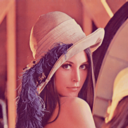
\includegraphics[width=64pt]{figures/reconstruction/lo128.png} & 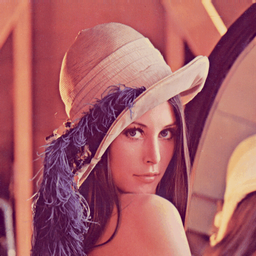
\includegraphics[width=64pt]{figures/reconstruction/lo256.png} & 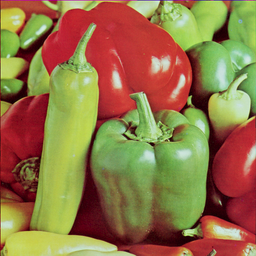
\includegraphics[width=64pt]{figures/reconstruction/po256.png}\\\hline
M = 50 & 
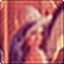
\includegraphics[width=64pt]{figures/reconstruction/lo6450.png} & 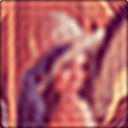
\includegraphics[width=64pt]{figures/reconstruction/lo12850.png} & 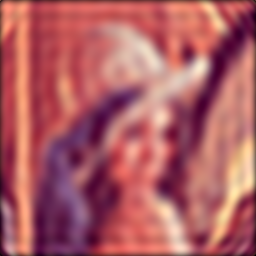
\includegraphics[width=64pt]{figures/reconstruction/lo25650.png} & 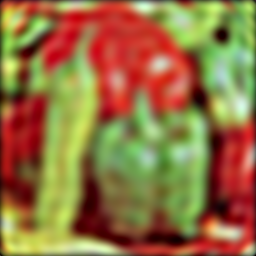
\includegraphics[width=64pt]{figures/reconstruction/po25650.png}\\
& 0.01257 & 0.01948 & 0.02659 & 0.03777\\
M = 100 & 

\includegraphics[width=64pt]{figures/reconstruction/lo64100.png} & \includegraphics[width=64pt]{figures/reconstruction/lo128100.png} & \includegraphics[width=64pt]{figures/reconstruction/lo256100.png} & \includegraphics[width=64pt]{figures/reconstruction/po256100.png}\\
& 0.00468 & 0.00719 & 0.01341 & 0.01596\\
M = 150 & & 
\includegraphics[width=64pt]{figures/reconstruction/lo128150.png} & \includegraphics[width=64pt]{figures/reconstruction/lo256150.png} & \includegraphics[width=64pt]{figures/reconstruction/po256150.png}\\
& & 0.00388 & 0.00868 & 0.00885\\
M = 250 & & & 
\includegraphics[width=64pt]{figures/reconstruction/lo256250.png} & \includegraphics[width=64pt]{figures/reconstruction/po256250.png}\\
& & & 0.00428 & 0.00378\\
M = 350 & & & 
\includegraphics[width=64pt]{figures/reconstruction/lo256350.png} & \includegraphics[width=64pt]{figures/reconstruction/po256350.png}\\
& & & 0.00279 & 0.00253\\
& \\

\end{tabular}
\caption{Reconstructed images using the old method, with the normalized mean squared error shown below each image.}
\label{fig:reconstruction_old}
\end{figure}

\begin{figure}
	\centering
\begin{tabular}{q | Q Q Q Q }
M & Lenna $64\times 64$& Lenna $128\times 128$ & Lenna $256 \times 256$ & Pepper $256 \times 256$\\ \hline\hline
Original & 
\includegraphics[width=64pt]{figures/reconstruction/lo64.png} & \includegraphics[width=64pt]{figures/reconstruction/lo128.png} & \includegraphics[width=64pt]{figures/reconstruction/lo256.png} & \includegraphics[width=64pt]{figures/reconstruction/po256.png}\\\hline
M = 50 &
\includegraphics[width=64pt]{figures/reconstruction/ln6450.png} & \includegraphics[width=64pt]{figures/reconstruction/ln12850.png} & \includegraphics[width=64pt]{figures/reconstruction/ln25650.png} & \includegraphics[width=64pt]{figures/reconstruction/pn25650.png}\\
& 0.00380 & 0.00901 & 0.01611 & 0.01778\\
M = 100 & 
\includegraphics[width=64pt]{figures/reconstruction/ln64100.png} & \includegraphics[width=64pt]{figures/reconstruction/ln128100.png} & \includegraphics[width=64pt]{figures/reconstruction/ln256100.png} & \includegraphics[width=64pt]{figures/reconstruction/pn256100.png}\\
& 0.01181 & 0.00246 & 0.00790 & 0.00681\\
M = 150 & & 
\includegraphics[width=64pt]{figures/reconstruction/ln128150.png} & \includegraphics[width=64pt]{figures/reconstruction/ln256150.png} & \includegraphics[width=64pt]{figures/reconstruction/pn256150.png}\\
& & 0.00152 & 0.00463 & 0.00349\\
M = 250 & & & 
\includegraphics[width=64pt]{figures/reconstruction/ln256250.png} & \includegraphics[width=64pt]{figures/reconstruction/pn256250.png}\\
& & & 0.00190 & 0.00131\\
M = 350 & & & 
\includegraphics[width=64pt]{figures/reconstruction/ln256350.png} & \includegraphics[width=64pt]{figures/reconstruction/pn256350.png}\\
& & & 0.00238 & 0.00229\\
& \\

\end{tabular}
\caption{Reconstructed images using the proposed new method, with the normalized mean squared error shown below each image.}
\label{fig:reconstruction_new}
\end{figure}

\begin{table}
    \centering
    \begin{tabular}{|c||c|c|c|c|c|}
        M & 50 & 100 & 150 & 250 & 350 \\ \hline
        old method $\varepsilon^2$ & 0.02659 & 0.01341 & 0.00868 & 0.00428 & 0.00279 \\ 
        new method $\varepsilon^2$ & 0.01611 & 0.00790 & 0.00463 & 0.00190 & 0.00238 \\ \hline
        change & -39.4\% & -41.1\% & -46.7\% & -55.6\% & -14.7\% \\
    \end{tabular}
    \caption{Comparison of the normalized mean squared errors between the two method, for the $256 \times 256$ Lenna image.}
    \label{tab:epsilons}
\end{table}

\section{Image recognition}

\section{Template matching}
